\textbf{{1.进程的创建}}

\textbf{(1)进程前趋图}\\
一个进程可以创建若干个新进程,新创建的进程又可以创建子进程,为了描述进程之间的创建关系,引入了下图所示的进程前趋图。

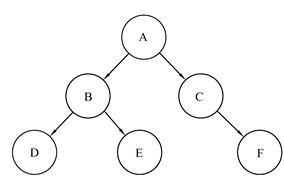
\includegraphics[width=2.95833in,height=1.95833in]{png-jpeg-pics/FE26B0A670DD08E1F9CF55E58FFA9A29.png}

\textbf{(2)创建原语}

在多道程序环境中,只有进程才可以在系统中运行。为了使一个程序能运行,必须为它创建进程。\textbf{导致进程创建的事件有:用户登录、作业调度、请求服务。}

{进程创建}{是通过创建原语实现的。其主要操}{作}{过程}{如下:}\\
\textbf{a.~}先向系统申请一个空闲PCB,并指定唯一的进程标识号PID。\\
\textbf{b.~}为新进程分配必要的资源。\\
\textbf{c.~}将新进程的PCB初始化。为新进程的PCB填入进程名、家族信息、程序数据地址、优先级等信息。\\
\textbf{d.~}将新进程的PCB插入就绪队列。

\textbf{{2.进程的撤销}}\\
导致进程撤销的事件有:进程正常结束、进程异常结束及外界干预等。

{撤销原语的功能是}{撤销一个进程}{,其主要操作过程如下:}\\
\textbf{a.~}先从PCB集合中找到被撤销进程的PCB。\\
\textbf{b.~}若被撤销进程正处于执行状态,则应立即停止该进程的执行,设置重新调度标志,以便进程撤销后将处理器分配给其他进程。\\
\textbf{c.~}对后一种撤销策略,若被撤销进程有子孙进程,还应将该进程的子孙进程予以撤销。\\
\textbf{d.~}回收被撤销进程所占有的资源,或者归还给父进程,或者归还给系统。最后,回收它的PCB。

\textbf{{3.进程的阻塞与唤醒}}\\
阻塞原语的功能是将进程由执行状态转为阻塞状态,而唤醒原语的功能则是将进程由阻塞状态变为就绪状态。{当一个进程期待的某一事件尚未出现时,该进程调用阻塞原语将自己阻塞起来。}{该进程自身调用原语阻塞自己的,是一种主动行为。}

{阻塞原语}{的主要操作}{过程}{如下:}\\
\textbf{a.~}首先停止当前进程的运行。由于该进程正处于执行状态,故应中断处理器。\\
\textbf{b.~}保存该进程的CPU现场以便之后可以重新调用该进程并从中断点开始执行。\\
\textbf{c.}
停止运行该进程,将进程状态由执行状态改为阻塞状态,然后将该进程插入到相应事件的等待队列中。\\
\textbf{d.~}转到进程调度程序,从就绪队列中选择一个新的进程投入运行。\\
对处于阻塞状态的进程,当该进程期待的事件出现时,由发现者进程调用唤醒原语将阻塞的进程唤醒,使其进入就绪状态。

\textbf{注意}:一个进程由\textbf{执行状态变为阻塞状态,是由这个进程自己调用阻塞原语去完成的;而进程由阻塞状态转变为就绪状态,则是由另一个发现者进程调用唤醒原语实现的,}一般这个发现者进程与被唤醒进程是合作的并发进程。
